\documentclass[conference=acm]{confpaper}

% General
% -------
\usepackage{pdflscape}
\usepackage{comment}
% Bibliography
% ------------
\bibliography{paper}

% Commands
% --------

\pgfsetarrows{latex-latex}
\tikzset{%
  base/.style = {inner sep=5pt,
                 text centered,
                 thin,
                 font=\rmfamily},
  round/.style = {base,
                  rectangle,
                  rounded corners=1ex,
                  draw=black,
                  fill=gray!20,
                  minimum height=0.35in}
}


%%%%%%%%%%%%%%%%%%%%  SPACE SAVINGS %%%%%%%%%%%%%%%%%%%%%%

\usepackage[all=normal,wordspacing]{savetrees}

%%%%%%%%%%%%%%%%%%%%  TITLE/AUTHORS  %%%%%%%%%%%%%%%%%%%%%

\title{A Comparative Analysis of Popular Video Conferencing Applications}

\author{ Authors }

\titlespacing\section{0pt}{*1.8}{*1.1}
\titlespacing\subsection{0pt}{*1.5}{*1.1}
\titlespacing\subsection{0pt}{*1.3}{*0.8}

%%%%%%%%%%%%%%%%%%%%  START OF DOCUMENT  %%%%%%%%%%%%%%%%%

\begin{document}

\abstract{
Video conferencing applications (VCAs) have become a critical Internet
application, even more so during the COVID-19 pandemic, as users worldwide now rely on them for
work, school, and telehealth. % COVID-19 has spurred unprecedented
%growth in the use of VCAs, with some Internet service providers seeing
%video conferencing traffic triple over an eight-month period
%in 2020. 
It is important to understand the resource requirements of different
VCAs and how these VCAs perform under different network conditions, including:
how much ``speed'' (specifically, upstream and downstream throughput) a VCA needs to support high quality of experience, how
VCAs perform under temporary reductions in available capacity; how they compete
with themselves, with each other, and with
other applications; and how usage modality (e.g., number of participants)
affects utilization.  We study three modern VCAs: Zoom, Google Meet,
and Microsoft Teams.   Answers to these questions differ substantially
depending on VCA.  First, the average utilization on an unconstrained
link varies between 0.8~Mbps and 1.9 Mbps.  Given temporary reduction of
capacity, some VCAs can take as long as 45 seconds to recover to average.  Differences in proprietary
congestion control also create unfair bandwidth allocations: in
constrained bandwidth settings, one Zoom video conference can consume more than 75\%
of the available bandwidth when competing with another VCA (e.g., Meet, Teams).  For some VCAs, client utilization can
decrease as the number of participants increases, due to the reduced video
resolution of each participant's video stream given a larger number of
participants. 
}



% Video conferencing has been one of the killer applications of the Internet. The video conferencing application (VCA) landscape has recently undergone significant change owing to the ongoing covid pandemic with the introduction of new VCA applications (e.g., Google Meet, Microsoft Teams) or revamping of incumbent VCA (e.g., Zoom, Bluejeans) to facilitate user engagement. The VCAs, however, have differed in their design choices and features. Understanding these differences with their impact on application performance and network consumptions can help in improving the design of future VCAs.  

% In this paper, we conduct extensive measurments contrasting the design differences for three popular VCAs, namely Zoom, Google Meet, and Microsoft Teams. We first study the application performance metrics in a 2-person call under different network conditions. We find that differences in application performance under same network conditions which can be attributed to differences in encoding mechanisms, application-level capping, bandwidth estimation techniques. We also found that performance varies across device platform even for the same application (e.g., native client better than the web client). We next study the impact of usage modality (e.g., gallery vs speaker mode in zoom) on network consumption and find some interesting differences in network consumption based on the usage modality. For instance, Zoom typically increases the sent video resolution of the user under speaker mode. Finally, we also study how different VCAs share bandwidth with other applications (file download, video streaming, and other VCAs) in terms of fairness. We find interesting differences wherein we find that applications do not share bandwidth fairly with other internet applications. 
% %A systematic understanding of the VCA design and its implications on network-levek performance is can be useful especially for improving the design of these services. In this paper, we conduct extensive measurements to understand and contrast the design of three popular VCAs, namely Zoom, Google Meet, and Microsoft Teams. 



%The video conferencing application (VCA) landscape has changed significantly because of COVID-19, with the introduction of new VCAs (e.g. Google Meet, Microsoft Teams) and renewal of incumbent VCAs (e.g. Zoom, Bluejeans). Because these VCAs differ in their design choices and features, it is critical that we understand how these differences impact application performance and network consumption under different network conditions and call modalities. This has two-fold advantages: i) a comparative analysis can uncover best design practices useful for improving current and future VCAs, and ii) understanding VCA network consumption for different contexts can be useful for ISPs in network provisioning and for telecommunication policy makers in defining benchmarks for Broadband access.   




%We find differences in VCA behavior under same static network conditions, such as different maximum (or nominal) bitrate (0.8 Mbps-1.9 Mbps) and inefficient network utilization for some VCAs under constrained links (e.g., 50\% for Meet). Next, we study how each VCA responds to dynamic network conditions by introducing (1) temporary bandwidth drops or (2) a competing application (e.g. Netflix, TCP iPerf3) on the same link. All require at least 20 seconds to return to their nominal sending rate following a temporary uplink constraint to 0.25Mbps. Further, Microsoft Teams is especially slow to recover from drop in downlink bandwidth because they do not do congestion control from the cloud. When competing with other applications on a constrained link, Zoom aggressively consumes available bandwidth, while Meet and Teams back off at low bandwidths. Finally, we investigate how usage modality (e.g. number of participants, speaker vs. gallery mode) affect consumption. Increasing the number of participants may reduce a user's network utilization. We find that a user's sending bitrate at least doubles when their video is pinned by all other participants. 

%All VCAs require at least 20 seconds to return to their nominal sending rate following a temporary uplink constraint to 0.25Mbps. Further, Microsoft Teams is especially slow to recover from drop in downlink bandwidth because they do not do congestion control from the cloud. When competing with other applications on a constrained link, Zoom aggressively can consume over 75\% of the available bandwidth when competing with Meet and Teams. 


\maketitle

\section{Introduction}\label{sec:intro}
COVID-19 has made video conferencing applications (VCAs) both common and necessary. People now regularly use VCAs for work, school, and telehealth, as activities have shifted from in-person to online. The success of remote communication indicates that VCAs will continue to play a critical role during and after the pandemic. However, VCAs are unique among internet applications and their increased use has altered the makeup of internet traffic. 

VCAs differ from other popular types of internet activity in several ways. Most notably, VCAs have far greater uplink utilization. Video streaming and internet browsing, two dominant sources of internet traffic, [receive the bulk of their traffic and send very little]. VCAs, however, send a video stream on the uplink. Further, VCAs do not benefit from network optimizations used in video streaming. Video streaming applications can "buffer" by fetching video ahead of time, then sporadically downloading when necessary. VCAs can not download video ahead of time because the video occurs in real-time. As a result, VCAs require a consistent and low-latency connection.

The earliest studies on VCAs focused on Skype, the dominant application in the VCA landscape at the time. These works sought to understand Skype from both a design and performance perspective. As the VCA landscape evolved over time, later work shifted their attention to newer VCAs and the protocols they used. 

While significant research and measurement studies have been conducted on VCAs in the past, both the VCAs and how we use them has since changed. Several new VCAs (e.g. Microsoft Teams, Google Meet) have been introduced, while existing VCAs (e.g. Zoom) have undergone a renewal. In light of these developments, it is important to investigate how differing VCA design choices impact application performance and network consumption. 


The continuing reliance on VCAs makes understanding these network requirements precisely crucial. In this paper, we conduct a comparative analysis of three popular VCAs: Google Meet, Microsoft Teams, and Zoom. We can determine these requirements by measuring VCA performance and consumption under realistic network conditions, including low bandwidth availability and other activity on the same network. Our goal is to understand the following:
\begin{enumerate}
    \item How VCAs performance varies under different static network conditions.
    \item How VCAs respond to temporary drops in bandwidth availability.
    \item How VCAs interact with competing applications on a constrained link.
    \item How usage modalities (number of participants, speaker vs. gallery viewing) affect network consumption.
\end{enumerate}

Answering the first question gives us insight into the minimum network requirements for each VCAs. 




% \begin{itemize}
% \item VCAs have been touted as a killer application for the Internet connecting millions of users. Significant research and measurement studies have been conducted benchmarking the VCAs of the time, their design choices and its impact on application performance. 

% \item The VCA application has undergone significant change in the covid-era of work from home/school with either new VCAs have been introduced or existing applications significantly revamped.

% \item In the context of these changes, it is important to revist the earlier measurement studies especially understanding how these changes relate to application performance and network consumption.

% \item In this paper we do a comparative analysis of three popular applications, namely zoom, meets, and teams. 

% \item Our analysis compares the VCAs along these three questions: i) How does the application performance vary under different network conditions?, ii) What is the impact of different VCA usage modality on network consumption, iii) Are the VCA applications fair in terms of bandwidth sharing when compared to other applications or transport protocols.

% \item Underlying question: what network conditions are required to support multiple streams through a link, at full performance?  Conversely, what network conditions are associated with degraded performance?  (Implications for broadband debates.)

% \item Insights: We find that ... 
% \end{itemize}

\section{Background \& Experiment Setup}
\label{sec:background}

We provide a brief background on video conferencing transport, technology, and
architecture before turning to our experiment setup.

\subsection{Video Conferencing Applications}

Most modern VCAs use Real-time Transport Protocol (RTP)~\cite{schulzrinne1996rtp,
schulzrinne2003rfc3550} or its variants~\cite{baugher2004secure, zoom_rtp} to
transmit media content. The audio and video data is generally transmitted over
separate RTP connections. RTP also uses two other protocols in conjunction,
Session Initiation Protocol (SIP)~\cite{rosenberg2002sip} to establish
connection between clients and RTP Control Protocol
(RTCP)~\cite{schulzrinne2003rfc3550} to share performance statistics and
control information during a call. Despite using well-known protocols, VCAs
can differ from each other significantly across the following dimensions:


\begin{itemize}
    \itemsep=-1pt
    \item \textbf{Network mechanisms}: RTP and the associated protocols are
        implemented in the application-layer. Thus, the specific
        implementation of the protocols can vary across VCAs. For instance,
        Zoom reportedly uses a custom extension of RTP~\cite{zoom_rtp}).
        Furthermore, the key network functions, i.e., congestion control and
        error recovery, can also be different and proprietary. 

    \item \textbf{Application-layer parameters}: These include media encoding
        standards and default bitrates. More recent video codecs (e.g., VP9,
        H.264) can encode at the same video quality with fewer bytes when
        compared to older codec (e.g., VP8), albeit with a higher compute
        overhead~\cite{bienik2016performance}. 
    
    \item \textbf{Streaming architecture}: VCAs can either choose to use
        direct connections or use relay servers. Centralized servers are
        almost always used for multi-point calls to combine data from multiple
        users. VCAs can differ in the exact strategies of data combination as
        well as the geographic footprint of their servers. For instance, Zoom
        rapidly expanded its server infrastructure to support increased call
        volume because of COVID-19~\cite{liu2020characterizing}. 

\end{itemize}
\noindent
Differences across one or more of these factors can lead to different VCA
network utilization and performance. In this paper, we aim to dig deeper into
some of these differences for a subset of VCAs. 


\subsection{Experiment Setup} 
\label{subsec:setup}

\paragraph{Video Conferencing Applications}:
In this paper, we study three popular VCAs---\zoom, Google \meet, and Microsoft \teams.
These VCAs have been used extensively worldwide over the past year, especially
in enterprises and educational institutions~\cite{vca_share}.  Teams and Zoom
provide desktop applications as well as browser clients, whereas Meet is ``native"
in the Chrome. Most of our tests are conducted using the desktop
applications for Teams and Zoom, and using the Google Chrome browser for Meet.
In-browser tests for Teams and Zoom are specified by \textit{\teamsbrowser}
and \textit{\zoombrowser}, respectively. We use Chrome (Meet) version
89.0.4389, Zoom client version 5.6.1, and Teams client version 1.4.00.7556.


\paragraph{Laboratory Environment}:
We conduct experiments in a controlled environment.  We begin by describing our experimental setup for a 2-party call. We use two identical laptops, referred to as C1 and C2, representing the two VCA clients. Each laptop is a Dell Latitude 3300 with a screen resolution of 1366 $\times$
768 pixels and running Ubuntu 20.04.1. The laptops have a wired connection to
a Turris Omnia 2020 router and access a dedicated 1~Gbps symmetric link
to the Internet.  Each experiment consists of a call between C1 and C2 under a
pre-specified network bandwidth profile and VCA. The bandwidth profile is
emulated by shaping the link between C1 and the router using traffic control
(\texttt{tc}). A pre-recorded talking-head video\footnote{It would be inappropriate to use the 
device webcam as the video, because without movement, VCAs compress the video
and ultimately send at a much lower rate than during a normal call.} with a
resolution of 1280 $\times$ 720 is used as the video source for the call, using \texttt{ffmpeg}.
This is done to both replicate a real video call and ensure consistency across
experiments. All experiments are conducted with the laptop lid open and the
application window maximized. 

\begin{figure*}[t!]
\begin{subfigure}[t]{0.33\textwidth}
    \centering
    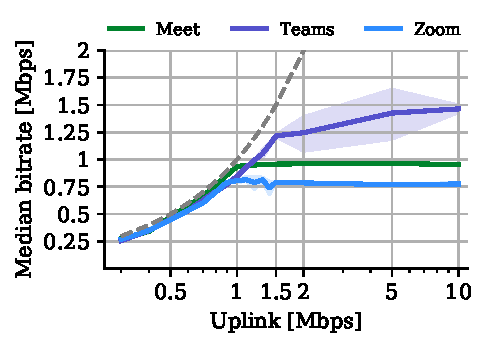
\includegraphics[width=\textwidth,keepaspectratio]{figures/static/uplink.pdf}
    \caption{Uplink bandwidth vs network bitrate %\jamie{label $x = y$}
    }
	\label{subfig:uplink_bitrate}
\end{subfigure}\hfill
\begin{subfigure}[t]{0.33\textwidth}
\centering
    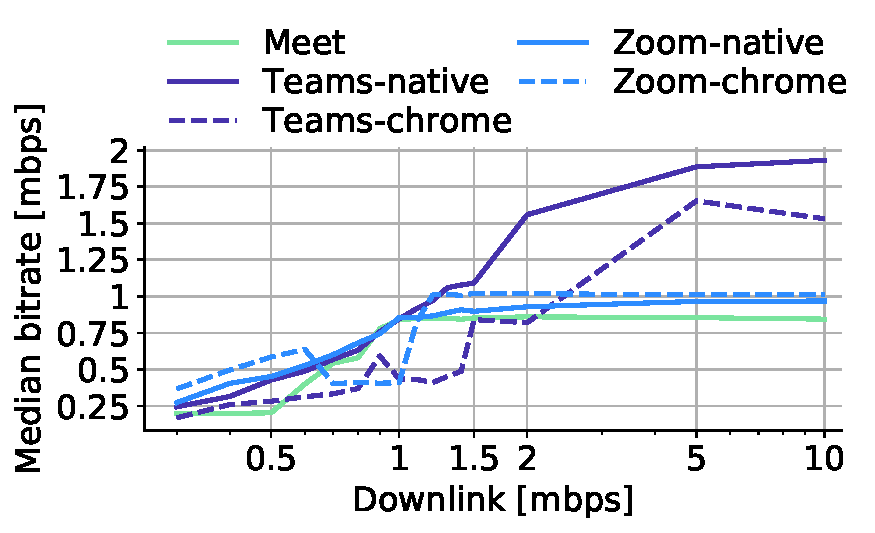
\includegraphics[width=\textwidth,keepaspectratio]{figures/static/downlink.pdf}
    \caption{Downlink bandwidth vs network bitrate}
	\label{subfig:downlink_bitrate}
\end{subfigure} \hfill
\begin{subfigure}[t]{0.33\textwidth}
\centering
    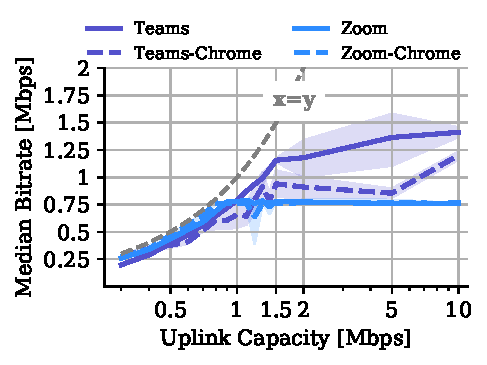
\includegraphics[width=\textwidth,keepaspectratio]{figures/static/uplink_browser.pdf}
    \caption{Impact of VCA platform %\jamie{capitalize Chrome}
    }
	\label{subfig:uplink_browser}
\end{subfigure} 
\vspace{-1em}
\caption{Utilization under different shaping levels. The bands represent 90\% confidence intervals.}
\label{fig:static}
\end{figure*}
%on the laptop and router for uplink and downlink shaping, respectively. During the competition experiments, all shaping occurs at the router.

\paragraph{Automating Experiments}: To conduct experiments at scale, we
automated the entire in-call process. We take several steps to recreate the
in-call process.  We use the Python PyAutoGUI package~\cite{pyautogui} to
automate joining and leaving calls. The package enables to programmatically
control the keyboard and the mouse by specifying coordinates or visual
elements on the screen. For \zoombrowser, we encountered CAPTCHA before
joining a call on the default browser. Using the Selenium-based Chrome
browser~\cite{selenium}, however, enabled us to bypass the CAPTCHA. Note the
experiments using Selenium are run exactly as it would be in default Chrome
browser. The workflow is controlled from C1, with TCP sockets used to
coordinate between C1 and C2.  We modify this setup slightly for subsequent
experiments (e.g., multi-party calls); those slight modifications are
described in the respective sections.


%%%%%%%%%%%%%%%%%



\begin{comment}
\paragraph{Performance metrics}: We mainly focus on the following application metrics. 
\begin{itemize}
    \item \textbf{Network bitrate}
    \item Video resolution
    \item Frames per second
    \item Freeze count
    \item Freeze duration
    \item Jitter-buffer delay 
\end{itemize}

Most of our analysis is using network bitrate. We consider other application performance metrics when they can be extracted from Google Chrome\footnote{chrome://webrtc-internals}. Our analysis shows that there is a strong correlation between network bitrate and application performance. This is intuitive as real-time streaming is characterized by low latency and thus any network interruptions usually lead to degradation in application performance. 


\subsection{Measurement Method}
  
The measurement setup consists of several components:

Hardware
\begin{itemize}
    \item matched laptops for nominal flows
          \begin{itemize}
              \item All Linux; caveats -- may not be the most-maintained apps
              \item What laptops, for the many-laptop tests?
          \end{itemize}
    \item turris router for control of single shaped link
    \item private iperf server on university network
\end{itemize}

\begin{itemize}
    \item traffic control scripts
    \item autogui; selenium for browser
          \begin{itemize}
              \item Important that we have the screen up -- see e.g., the tweet, but maybe chase the paper, about the struggle of getting the machines to actually render flows being important.
              \item client vs browser
              \item sw versions?
          \end{itemize}
    \item pcap, iperf logs
    \item webrtc
          \begin{itemize}
              \item difference between meet and zoom 
          \end{itemize}
    \item Zoom API access (\& limitations?)
    \item control over sockets?
\end{itemize}

\begin{table*}[t!]
\centering
\begin{tabular}{|c|c|c|c|c|}
\hline
\paragraph{VCA} & \textbf{Platforms}     & \textbf{Encoding} & \textbf{Direct connection?} & \textbf{Network Protocol} \\ \hline
\hline 
Meet  & Browser, Phone         & VP9/VP8   & No                 & RTP (WebRTC)     \\ \hline
Teams & Native, Browser, Phone & VP9       & ?                  & RTP              \\ \hline
Zoom  & Native, Browser, Phone & H.264 SVC & Yes                & Variation of RTP \\ \hline
\end{tabular}
\caption{Design parameters of selected VCAs}
\label{tab:vca_overview}
\end{table*}
\end{comment}


\section{Performance on Different Networks}\label{sec:methodology}
We begin by measuring how VCAs perform under different network conditions. 
In the first set of experiments, we study the impact of \textbf{bandwidth}, \textbf{latency}, 
and \textbf{loss} on application performance. In the second set of experiments, 
we analyze how these applications respond to new flows on the network.
\subsection{Static Network Conditions}


\noindent\textbf{Methodology}. 


\subsection{Dynamic Network Conditions}

\subsubsection{Temporary Interruptions}

\noindent \textbf{Methodology}.

\subsubsection{Competing Flows}

\noindent \textbf{Methodology}.



\section{Application context and network consumption}\label{sec:usage_modality}
In this section, we analyze the impact of different usage modalities such as the number of persons in the call, viewing mode, and device type on the network consumption. 
\subsection{Number of Users}
\subsection{Viewing Mode}

%\section{Performance and Fairness with Competing Flows}

\begin{figure}[]
    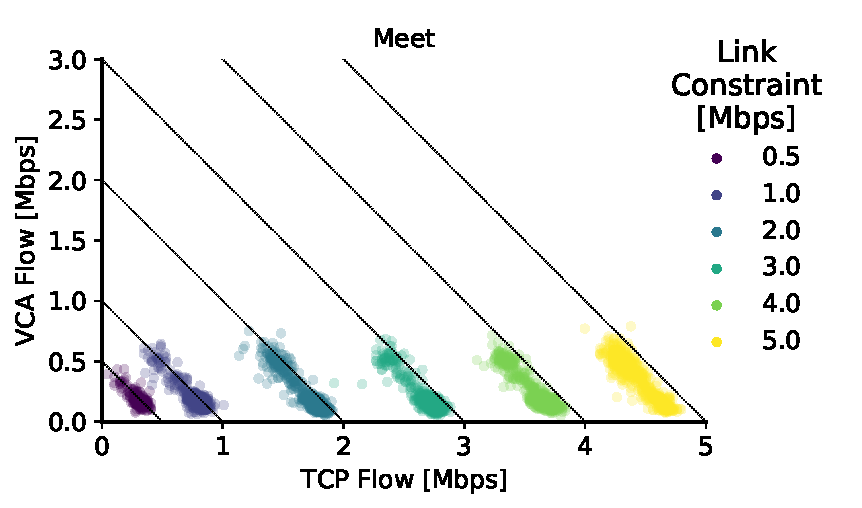
\includegraphics[width=\linewidth]{comp/meet_iperf_scatter.pdf}
    \caption{Competition between Meet and an iperf3 TCP flow.}
	\label{fig:comp_meet_iperf}
\end{figure}

\begin{figure}[]
    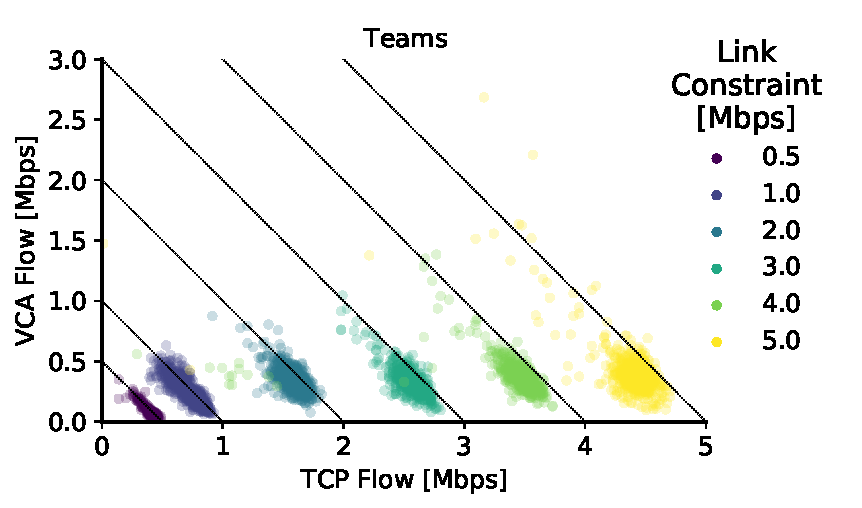
\includegraphics[width=\linewidth]{comp/teams_iperf_scatter.pdf}
    \caption{Competition between Teams and an iperf3 TCP flow.}
	\label{fig:comp_teams_iperf}
\end{figure}

\begin{figure}[]
    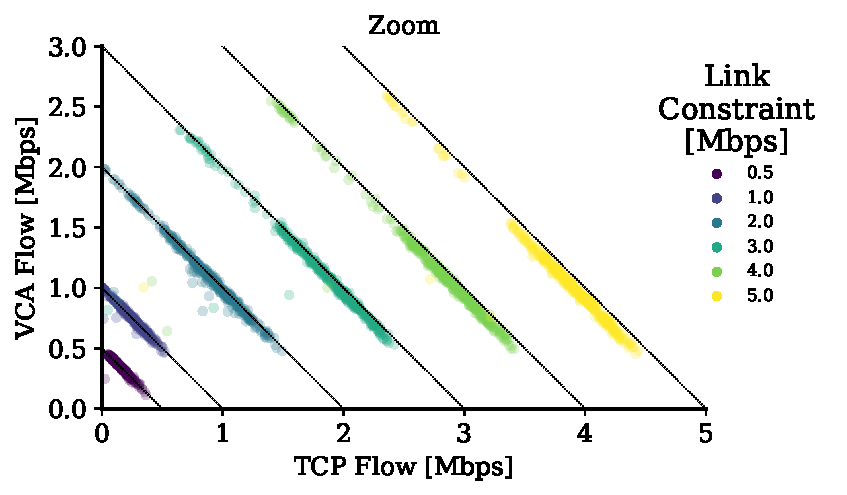
\includegraphics[width=\linewidth]{comp/zoom_iperf_scatter.pdf}
    \caption{Competition between Zoom and an iperf3 TCP flow.}
	\label{fig:comp_zoom_iperf}
\end{figure}

\begin{figure}[]
    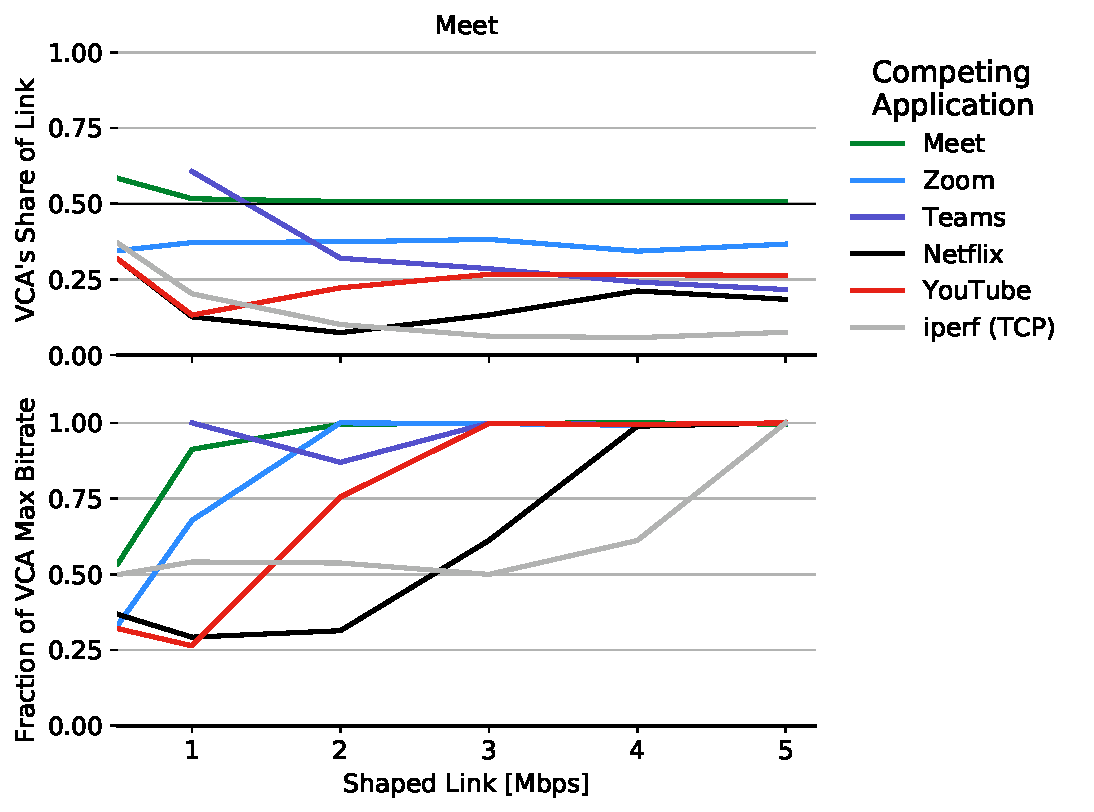
\includegraphics[width=\linewidth]{comp/meet_competition.pdf}
    \caption{Link share and share of nominal bitrate for Meet, in competition with other flows, as a function of downlink bitrate cap}
	\label{fig:meet_comp_bitrates}
\end{figure}

\begin{figure}[]
    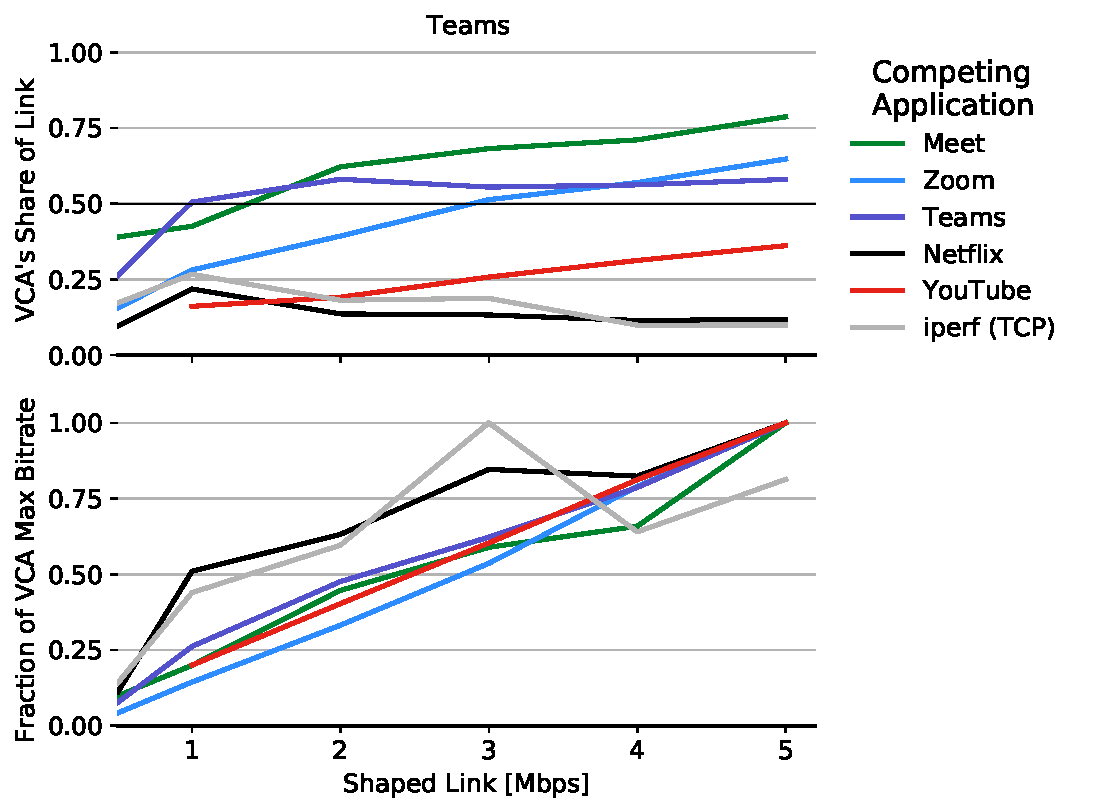
\includegraphics[width=\linewidth]{comp/teams_competition.pdf}
    \caption{Link share and share of nominal bitrate for Teams, in competition with other flows, as a function of downlink bitrate cap}
	\label{fig:teams_comp_bitrates}
\end{figure}

\begin{figure}[]
    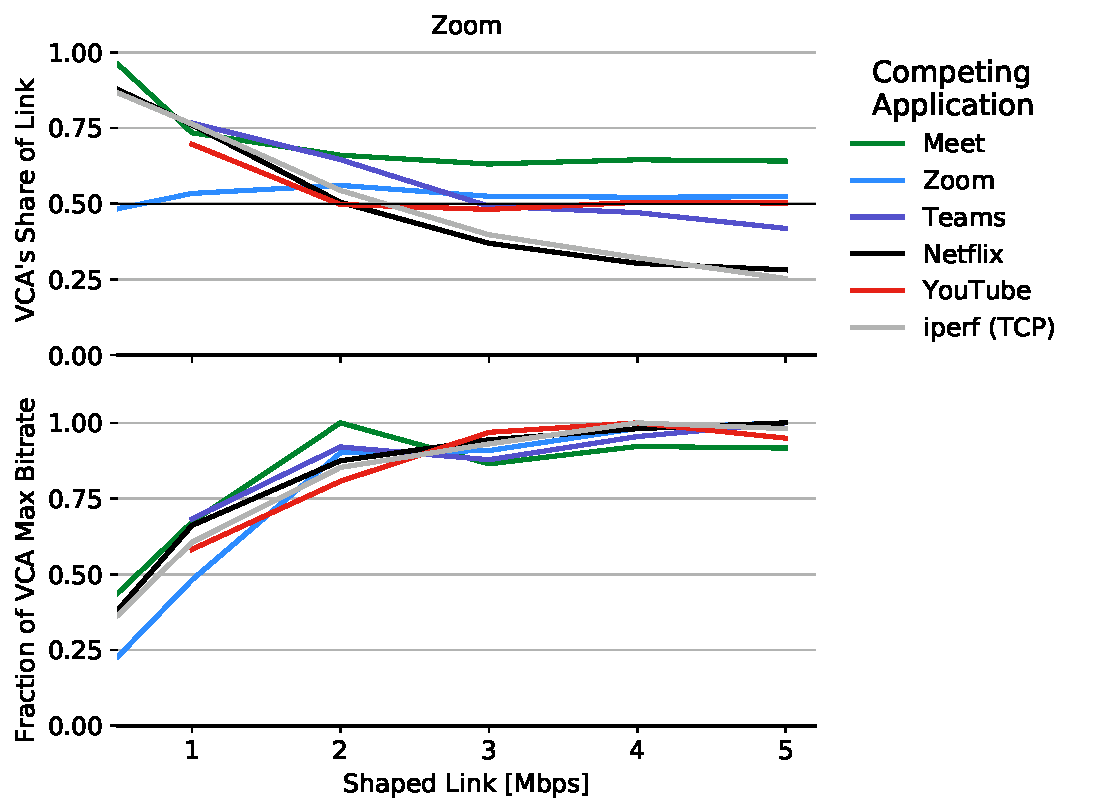
\includegraphics[width=\linewidth]{comp/zoom_competition.pdf}
    \caption{Link share and share of nominal bitrate for Zoom, in competition with other flows, as a function of downlink bitrate cap.}
	\label{fig:zoom_comp_bitrates}
\end{figure}

\begin{figure}[]
    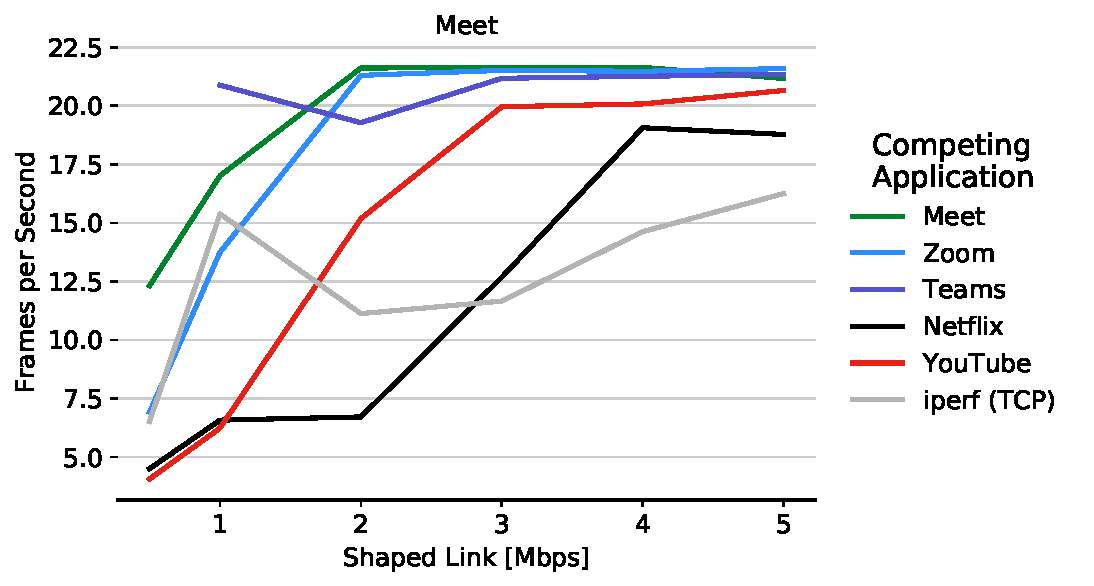
\includegraphics[width=\linewidth]{comp/meet_performance.pdf}
    \caption{Meet frames per second, in competition with other flows and as a function of link capacity.}
	\label{fig:meet_comp_performance}
\end{figure}

\begin{figure}[]
    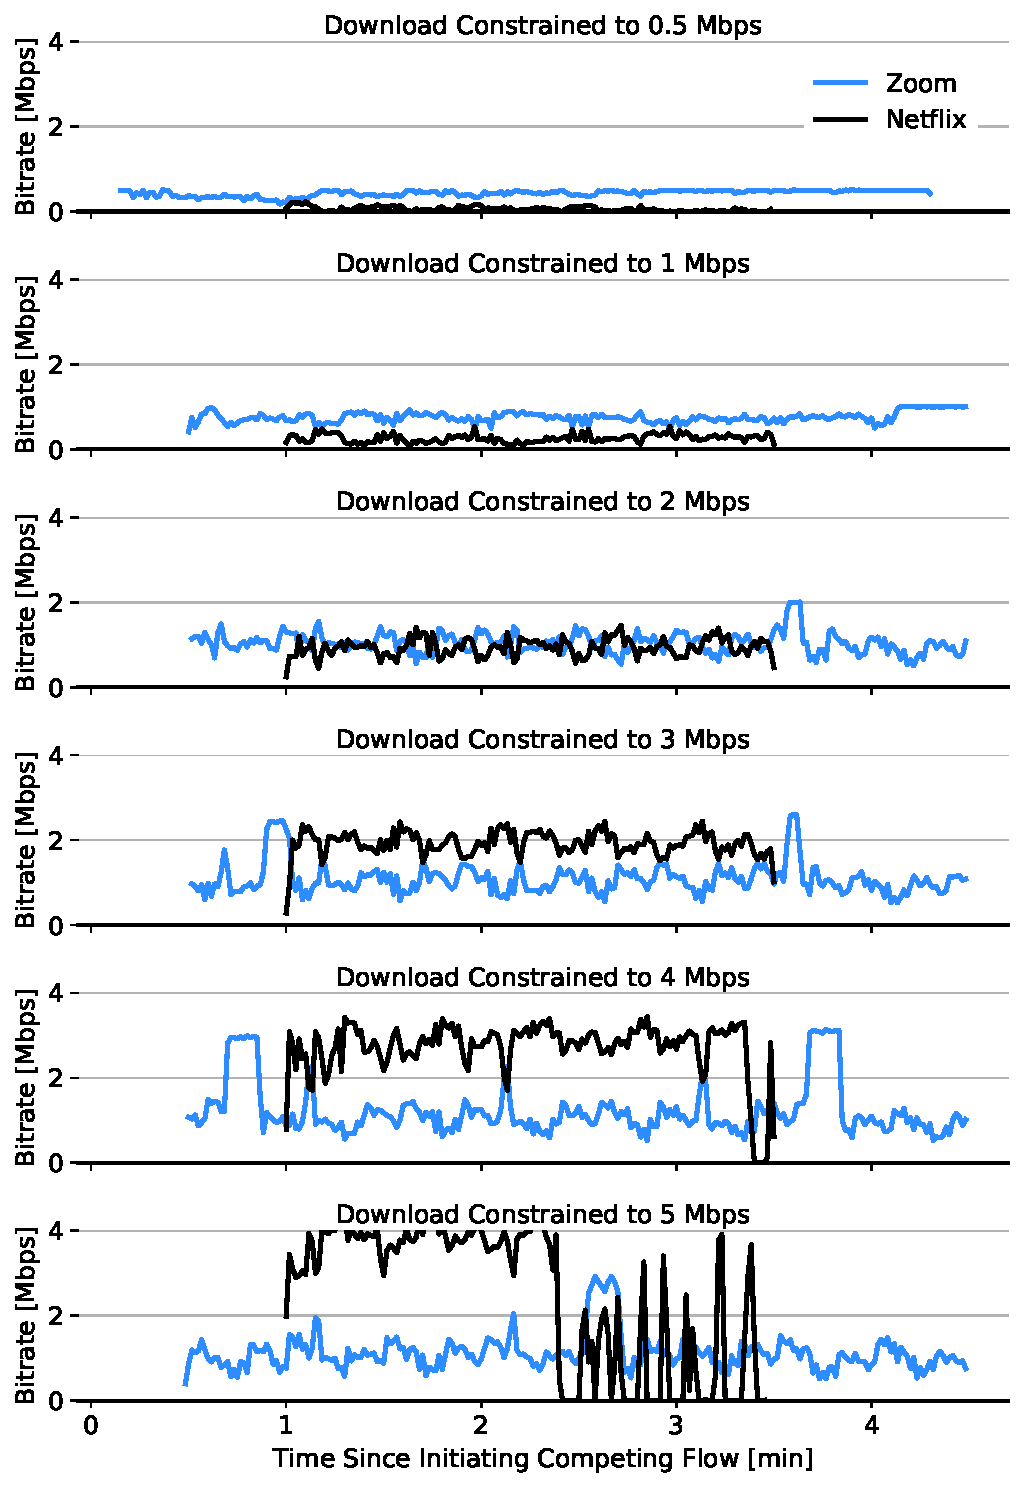
\includegraphics[width=\linewidth]{comp/zoom_netflix_dl_time_series.pdf}
    \caption{Time series of bitrate for Zoom in competition with a Netflix flow, at different link capacity.}
	\label{fig:ts_zoom_netflix}
\end{figure}

\section{Related Work}\label{sec:related}

\textbf{VCA measurement}: Some of the early VCA measurement work has focused on uncovering the design of the Skype focusing on its streaming protocols~\cite{baset2004analysis}, architecture~\cite{guha2005experimental}, traffic characterization~\cite{bonfiglio2008tracking}, and application performance~\cite{hossfeld2008analysis}. More recent work has included other VCAs and streaming contexts~\cite{xu2012video, yu2014can, azfar2016android}. Xu et al.~\cite{xu2012video} use controlled experiments to study the design and performance of Google+, iChat, and Skype. The work is further extended to include performance of the three services on mobile video calls~\cite{yu2014can}. 

Closest to our work is work by Jansen et al.~\cite{jansen2018performance} and Nistico et. al~\cite{nistico2020comparative}. Jansen et al. evaluate WebRTC performance using their custom VCA under controlled network conditions~\cite{jansen2018performance}. Emulating similar network conditions, we consider performance of commercial and more recent VCAs that widely used for education and work. Even between tested VCAs using WebRTC, namely \meet and \teamsbrowser, we find significant performance differences, likely due to different design parameters (e.g., codecs, default bitrates). Nistico et al.~\cite{nistico2020comparative} consider a wider range of recent VCAs, focusing on their design differences including protocols and architecture. Our work provides a complimentary performance analysis for a subset of the VCAs studied by them. We use the insights from their work to explain the differences among VCAs' network utilization and performance under similar streaming contexts. 

\textbf{VCA congestion control}: Several congestion control algorithms have been proposed for VCAs. These algorithms rely on a variety of signals such as loss~\cite{handley2003tcp}, delay~\cite{carlucci2016analysis}, and even VCA performance metrics~\cite{singh2012rate} for rate control. For instance, Google Congestion Control~\cite{carlucci2016analysis}, also implemented in WebRTC, uses one-way delay gradient for adjusting the sender rate while SCReAM~\cite{johansson2015self} relies on both loss and delay along with TCP-like self-clocking. %Salsify~\cite{fouladi2018salsify}, proposes a new approach to congestion control through a integration between congestion control and video encoding. 
While the VCAs may use one or more of these variants, the exact implementation of the algorithm and parameter values vary and is proprietary. In this work, we study the efficacy of the VCA congestion control in the case of transient interruptions and background applications. A recent study by Sander et al. evaluates \zoom's congestion control along these dimensions~\cite{sandervideo}. Our work observes similar results for \zoom and also analyses more VCAs, including their fairness to each other and other popular internet applications, namely YouTube (UDP-based) and Netflix (TCP-based). 


\begin{comment}
\textbf{Performance of Internet applications}
There is also related work on measuring other applications over the Internet including video streaming~\cite{}, web browsing~\cite{}, and online gaming~\cite{}. Our work focuses on VCAs which are characterized by their strict latency requirements and upstream link utilization.  
\end{comment}

\label{lastpage}
\section{Conclusion}\label{sec:conclusion}


\microtypesetup{protrusion=false}

\newpage
\printbibliography

\vfill
\pagebreak

\end{document}

%%%%%%%%%%%%%%%%%%%%  END OF DOCUMENT  %%%%%%%%%%%%%%%%%%%%
